\documentclass[11pt]{article}
\usepackage[margin=1.1in]{geometry}
\usepackage{amsmath,amssymb,graphicx,booktabs}
\usepackage[hidelinks]{hyperref}

\title{The Generative Ledger: A Derived Two-Queue Law Unifying the\\
Chronic and Acute Regimes of a Discrete Emergent Universe}
\author{Jason Merwin\\
\small Independent Researcher, Ashland, Oregon\\
\small (Simulations and analysis performed with AI assistance; see Acknowledgments)}
\date{July 2026 --- DRAFT v2 (merged)}

\newcommand{\dt}{\Delta t}

\begin{document}
\maketitle

\begin{abstract}
We report a quantitative experimental study of the load economics of a discrete
generative substrate: a growing, degree-regulated triangulated foam in which
update capacity is finite, locally boundary-counted, and genuinely contended. A
persistent defect (``mass'') imposes chronic computational demand; the scheduler
defers what it cannot serve, and deferred obligations accumulate as a literal
backlog. In the first part of this paper we measure this economy with
pre-registered predictions throughout: (i) without relief, chronic overload
produces a graded starvation continuum; (ii) in units of measured free capacity
the 50\%-collapse threshold is a dimensionless constant, $x_{50}=1.30$,
blind-confirmed on a held-out geometry; (iii) a manifold-legal topological
relief valve matches an oracle deletion valve's stitch law and exceeds its
stability; (iv) the same frozen engine exhibits an acute ``render gate'' and
(v) a complete Zeno-pattern suppression law. In the second part we go beyond
measurement. A pre-registered waveform-plane campaign shows the relieved
economy's collapse wall is a single dimensionless constant
($x_{50}\approx3.5$--$3.7$), invariant across pulse period up to $\dt=5$,
across three independent seed cohorts, and across exterior capacity exponents
$p\in\{0.6,0.75,0.9\}$; above $\dt=5$ the wall lifts along a measured knee
ramp. Event-level instrumentation then yields the relief valve's transfer
function as an \emph{exact} law, $n = 2\lceil\max(1,\lfloor \mathrm{pop}/6
\rfloor)/2\rceil$ (4227/4230 events), whose $1/6$ gain is derived from the
quota arithmetic and whose quantum of 2 is derived from the topology of the
collapse move. A five-rule two-queue reduction built from this derived gain and
per-run measured capacities---with zero fitted parameters---reproduces
individual run outcomes at 95--98\% and derives the chronic wall, the
waveform-invariant band, and the burst-stabilization endpoint within
measurement confidence intervals; two information variants of the reduction
bracket every measured wall, bounding a $\pm3\%$ residue attributed to
enumerated service microstructure. The chronic (gravitational-regime) and
acute (collapse-regime) phenomenologies of the model are thereby exhibited as
two operating regimes of one derived law. All claims are internal to the
model. We report our negative results, registered failures, and retractions
with the same prominence as our positive results; three consecutive registered
failures are, in fact, how the two-queue structure was found.
\end{abstract}

\section{Introduction and scope}
The Discrete Emergent Universe (DEU) program models spacetime as the output of
a finite generative process: a graph substrate updated by a scheduler with
bounded bandwidth \cite{rmr,foam,gbr,cga,qpc}. Earlier work in this program
proposed that gravitational phenomena correspond to chronic consumption of
local update bandwidth by persistent defects, and that
quantum-measurement-like phenomena correspond to acute saturation events.
Those proposals were made with varying degrees of rigor; several supporting
calculations in earlier drafts are superseded or retracted by the present work
(Section~\ref{sec:neg}).

This paper does two things carefully. First, it \emph{measures} the economics:
we freeze a single engine---substrate, scheduler, and relief mechanism---and
characterize its response to chronic, acute, and temporally structured load,
using pre-registered predictions and held-out confirmations wherever a
quantitative claim is made (Sections~\ref{sec:chronic}--\ref{sec:acute}).
Second, it \emph{derives} the economics: Section~\ref{sec:law} reduces the
engine to a five-rule two-queue law whose one internal constant is derived
rather than measured, and adjudicates that reduction against every measured
wall in the study with zero fitted parameters. The unification of the two
regimes, pre-registered as a conjecture in an earlier draft of this paper, is
reported here as a result.

\paragraph{Scope discipline.} Every claim in this paper is a claim about the
model. Where a result is structurally reminiscent of a physical phenomenon
(gravitational collapse, wavefunction collapse, the quantum Zeno effect), we
say ``analog'' or ``pattern'' and mean only that the mathematical shape of the
model's law matches the shape of the physical law. No claim of correspondence
with nature is made or implied. We adopt this discipline because the
alternative---announcing physics from internal consistency---is the
characteristic failure mode of speculative frameworks, including earlier
iterations of this one.

\section{The engine}
\subsection{Substrate}
The substrate is a growing triangulated 2-complex. Faces carry a refinement
depth $k$; a face of depth $k$ has weighted area $3^{-k}$ and weighted edge
length $3^{-k/2}$, so total weighted area is conserved under the
$1{\to}3$ refinement move. Face types $\{S,I,G\}$ drive growth through a
frustration rule ($S$ faces with a $G$ neighbor and no $I$ neighbor split);
child types are assigned by random permutation. Degree regulation is provided
by 2--2 edge flips accepted only when they reduce the local cost
$\sum_v(\deg v-6)^2$ and join faces of equal depth.

Both substrate rules were forced by measurement, not chosen a priori. Sorted
type assignment concentrates half of all faces on a single immortal vertex
(degree 6{,}318 of 12{,}636 faces in a reference run), destroying all metric
structure. Depth-unrestricted flips collapse the weighted diameter to
$\approx0.53$ at every flip cadence tested: a flip joining unequal depths
rewires adjacency across scales and acts as a metric wormhole. With both
constraints imposed, the vacuum passes its geometric entrance exam:
ball-growth dimension $d=2.00\pm0.11$ across seeds at $\sim3\times10^4$ faces,
weighted diameter 1.0--1.5, maximum vertex degree bounded at 25--28.

We state the design law these constraints exemplify, because it has now
recurred independently \emph{five} times in this program (flips, excision
scale, collapse orientation, observable definition, and---in
Section~\ref{sec:t1}---instrument timing):
\begin{quote}
Every legal move, and every observable, must respect the structure of the
metric it acts on---its scale, its radial fibration, its material identity,
\emph{and its timing relative to the events it measures}. Metric-blind moves
destroy emergent geometry; coordinate-fixed observables misread material
surgery; event-blind instruments misread their own mechanism.
\end{quote}

\subsection{Native scheduler}
A core window $W$ of weighted radius $r_c$ surrounds the defect anchor. Its
per-epoch capacity is $\Gamma$, the live count of its boundary edges---counted
by the scheduler at runtime, never supplied as a parameter. Forced defect
operations and vacuum maintenance (frustrated splits) compete for $\Gamma$ in
randomized order; unserved forced operations persist as a literal backlog $B$.
The exterior runs on a sub-extensive global budget $N^{3/4}$ (a declared
simplification). Sub-extensive capacity is itself empirically forced: with
extensive capacity the defect accelerates local activity and the starvation
channel inverts sign; positive time-dilation-like response exists only for
capacity exponents $p\lesssim0.75$.

\subsection{Relief valve}
When $B\ge\Gamma$, one relief event fires. Two mechanisms are compared: an
oracle (delete $\lfloor T/6\rfloor$ of the $T$ deepest defect faces by fiat)
and the collapse valve: link-conditioned edge collapses \cite{hoppe}
restricted to circumferential defect--defect edges at the defect's own metric
scale, voiding one deferred obligation per removed defect face. In
$>10^4$ executed collapses across all experiments the edge-incidence audit
recorded zero manifold violations.

\subsection{Instrumented variants and certification}\label{sec:instruments}
Sections~\ref{sec:acute}--\ref{sec:law} required event-level observables not
present in the base engine's log. Each instrumented variant (v21i: tagged
population and per-event voiding; v21i2: population read \emph{at trigger};
v21i3: standing vacuum demand) adds only pure reads---no dynamics, no random
draws. We adopted the rule that \emph{instruments are engines}: every variant
must reproduce, bit-exactly, a fixed panel of ten archived runs spanning both
load regimes, both outcome classes, and the extremes of the capacity lottery,
across all four scalar observables, before any of its data are used. All
variants passed 10/10; certification scope (scalar pipeline observables) is
declared, and geometry-sector claims from these variants are out of scope.

\subsection{Reproducibility}
All engines are deterministic given a seed. Code, per-run data, pre-registration
documents with frozen timestamps, and the continuity ledger sufficient to
reproduce every table and figure are provided in the supplementary archive.

\section{Methods: measures, metrics, and pre-registration}\label{sec:methods}
Three methodological rules produced every surviving result and caught every
retracted one. (1) \textbf{Declared measures}: on a multi-scale foam,
node-count, face-count, area-weighted, and length-weighted statistics of the
``same'' quantity differ by orders of magnitude; one early
``geometry-collapse'' finding was an artifact of switching measures between
sessions and is retracted in Section~\ref{sec:neg}. This campaign forced a new
clause: an observable must also declare its \emph{timing} relative to the
event it measures (served vs.\ demanded; pre-trigger vs.\ post-relief).
Section~\ref{sec:t1} documents the violation that forced the clause---committed
by the present authors, caught by pre-registration---and retains the affected
dataset as a methods specimen. (2) \textbf{Pre-registration}: quantitative
predictions and fit procedures were frozen before the runs that tested them;
amendments are permitted only with the prior failure and its diagnosis on the
record first. (3) \textbf{Bookkeeping identities as instrument checks}: the
measured late-time backlog slope equals $m-\bar s_F$ to within a few percent
in every cell of every sweep.

The primary chronic observable is the late-window backlog slope; a run is
classified \emph{runaway} if the slope exceeds 1 op/epoch over epochs 70--100.
The primary relief observable is the stitch count $k$. The dimensionless load
coordinate used throughout is
\begin{equation}
x=\frac{m}{\Gamma-D_{\mathrm{vac}}},
\label{eq:x}
\end{equation}
with $\Gamma$ and $D_{\mathrm{vac}}$ measured per run (late-window means).
Threshold fits are maximum-likelihood logistic; confidence intervals are
2000-resample bootstraps (fixed rng seed), resampled at the run level where
events within a run are correlated.

\section{Chronic load: the gravitational-regime economy}\label{sec:chronic}
\subsection{Gravity without relief: a graded starvation continuum}
With the valve disabled, chronic load $m$ produces neither stability nor a
binary collapse but a continuum of partial starvation. The normalized
starvation fraction $s=\mathrm{slope}/m$ occupies the middle band
$0.2<s<0.8$ in 43--70\% of runs at every load, with an atom of total
starvation ($s=1$; 7--27\%) and a persistent survivor tail (3--13\% fully
balanced even at $m=42$). An earlier ``bistable death spiral'' reading from
$n=8$ pilot statistics is retracted; the $n=30$ distributions are unimodal
with heavy endpoint structure. Within cells at fixed load, outcome correlates
strongly with each run's own native capacity: the seed lottery is a capacity
lottery. (Section~\ref{sec:u1} quantifies this: the per-run coordinate of
Eq.~\ref{eq:x} predicts individual outcomes at AUC 0.98--0.999 on three
independent seed cohorts.)

\subsection{The dimensionless collapse constant (no relief)}
Raw collapse thresholds differ across window geometries ($m_{50}=4.7$ and
$5.6$ at $r_c=0.06$ and $0.12$). Normalizing by gross capacity fails to
reconcile them (ratio 1.21); normalizing by free capacity
(Eq.~\ref{eq:x}) collapses both onto $x_{50}=1.30$ exactly. A pre-registered
falsification test on a third geometry ($r_c=0.20$), run blind with the fit
procedure frozen, gave
\begin{equation}
x_{50}=1.29,\quad 95\%\ \mathrm{CI}\ [1.17,1.45]\quad(\text{prediction: }1.30).
\end{equation}
The no-relief economy tolerates a chronic overload of ${\approx}30\%$ of its
free capacity before collapse odds reach one half, independently of window
geometry.

\subsection{Relief: two valves, one law, unequal margins}
A matched dual-arm sweep (30 seeds, $m\in\{4,\dots,34\}$, identical trigger)
adjudicates the collapse valve against the oracle (Table~\ref{tab:adjud},
Fig.~\ref{fig:valve}). Both arms obey the same stitch-rate law,
$k\propto m^{0.57}$, with absolute counts agreeing within ${\sim}5\%$ at every
load. Their stability margins differ: $m_{50}=26.2$ (collapse valve)
vs.\ 19.5 (oracle). Relative to the no-relief economy ($m_{50}\approx5$),
relief extends the stable regime by a factor of ${\sim}4$. The valve maintains
a genuine limit cycle with a persistent defect: tagged population oscillating
between 59 and 177 faces over fifty epochs while backlog repeatedly returns to
zero---relief, not annihilation. (We note for Section~\ref{sec:law} that the
$0.57$ exponent fits were taken at loads where the per-epoch relief cap
begins to censor $k$; a below-ceiling refit is registered future work.)

\begin{table}[t]
\centering\small
\begin{tabular}{r cc cc}
\toprule
 & \multicolumn{2}{c}{oracle} & \multicolumn{2}{c}{collapse valve}\\
$m$ & $P$ & $\bar k$ & $P$ & $\bar k$\\
\midrule
4  & 0.07 & 13.3 & 0.00 & 14.0\\
8  & 0.10 & 21.1 & 0.00 & 22.9\\
12 & 0.13 & 26.4 & 0.20 & 29.0\\
16 & 0.33 & 30.9 & 0.23 & 34.7\\
20 & 0.53 & 35.7 & 0.23 & 37.8\\
26 & 0.63 & 39.3 & 0.53 & 43.0\\
34 & 0.80 & 44.5 & 0.70 & 46.4\\
\midrule
fits & \multicolumn{2}{c}{$m_{50}=19.5$; $k\propto m^{0.57}$} &
       \multicolumn{2}{c}{$m_{50}=26.2$; $k\propto m^{0.57}$}\\
\bottomrule
\end{tabular}
\caption{Valve adjudication sweep, $r_c=0.06$, 30 seeds per cell. $P$ =
probability of runaway; $\bar k$ = mean relief events.}
\label{tab:adjud}
\end{table}

\subsection{The relieved constant and its universality}\label{sec:u4r}
The relieved economy has its own wall. On a fresh seed cohort (141--160) under
pure chronic load, the relieved threshold in free-capacity units is
$x_{50}=3.52$, 95\% CI $[3.37,3.71]$, consistent with the value obtained
independently from pulse-train schedules on a different cohort
($3.72$, $[3.60,3.87]$; Section~\ref{sec:u1}). A pre-registered three-arm test
then varied the exterior capacity exponent, $p\in\{0.6,0.75,0.9\}$, same
seeds and loads. Raw fragility differs wildly across arms (at $m=32$,
$P(\text{runaway})=0.85$ at $p=0.6$ vs.\ $0.50$ at baseline) because the
exterior exponent changes the substrate the window grows in (mean free
capacity 6.4/10.5/8.0); the dimensionless wall does not move:
$x_{50}=3.53\,[3.41,3.62]$, $3.52\,[3.37,3.71]$, and $3.45\,[3.37,3.56]$
(Fig.~\ref{fig:relieved}). The registered caveat that the starvation channel
might invert at $p\approx0.9$ did not fire. \textbf{The relieved constant
(${\approx}3.5$ in free-capacity units) is a constant of the mechanism class,
not of the exterior scheduling exponent.} The small spread between the
pulse-train estimate (3.72) and the chronic-arm cluster (3.45--3.53), with
overlapping CIs throughout, is a possible schedule effect and is flagged as a
consolidation item, not claimed either way.

\section{Acute and structured load: the collapse-regime economy}\label{sec:acute}
The engine, valve, trigger, and all constants are frozen from
Section~\ref{sec:chronic}; only the exogenous load schedule changes.

\subsection{The render gate}
Single-epoch spikes of total action $A$ produce no topological response below
a threshold and a graded burst above it (Fig.~\ref{fig:gate}).
Pre-registered onset $A^*\approx s+\Gamma$ predicts $A^*\approx23$; measured
onset 15--20, within seed scatter. Above onset, $\bar k$ rises from 0.6
($A=20$) to 7.0 ($A=150$) while clearing time grows only from 2 to 8 epochs:
denser stitch bursts, not longer sieges. A spike of $A=150$ always clears;
the equivalent chronic load kills a quarter of runs.

\subsection{Zeno-pattern suppression}
Fixing total action $A_{\rm tot}=60$ and subdividing into $N$ pulses:
\begin{center}\small
\begin{tabular}{l ccccccc}
schedule & $1{\times}60$ & $2{\times}30$ & $4{\times}15$ & $6{\times}10$ &
$10{\times}6$ & $15{\times}4$ & $30{\times}2$\\
$\bar k$ & 3.4 & 2.4 & 0.8 & 0.6 & 0.0 & 0.0 & 0.0\\
\end{tabular}
\end{center}
The suppression is monotone and complete (Fig.~\ref{fig:zeno}), exactly as
pre-registered: once each pulse can be serviced below the trigger line before
the next arrives, no sector is ever dropped. The temporal structure of action
delivery alone determines whether topology changes. We name it Zeno-pattern
suppression from bandwidth economics and claim nothing further.

\subsection{One wall across the waveform plane, and a knee}\label{sec:u1}
A pre-registered waveform-plane campaign (loads $\bar m\in\{16,\dots,40\}$,
periods $\dt\in\{1,2,4,8\}$, 20 seeds; extended to $\dt\in\{5,6,7\}$ on a
fresh cohort) tested whether the chronic wall is waveform-invariant. Three
results (Fig.~\ref{fig:knee}):

\emph{(a) The reduction generalizes.} The per-run coordinate
$x=\bar m/(\Gamma-D_{\rm vac})$ classifies individual runaways at AUC
0.979--0.999 on all cohorts, versus 0.59--0.66 for raw load. The chronic
outcome of an individual run is essentially determined by its own free
capacity---the capacity lottery, quantified.

\emph{(b) Waveform invariance holds through $\dt=5$.} Thresholds at
$\dt=1,2,4$ are statistically one number (pooled $x_{50}=3.72$,
$[3.60,3.87]$); matched-pair tests against the chronic arm are null at
$\dt=2,4$. A fresh-cohort point at $\dt=5$ ($3.69\,[3.50,4.03]$) sits on the
same band.

\emph{(c) Above $\dt=5$ the wall lifts along a graded ramp:} $4.16\,[3.94,4.38]$
at $\dt=6$, $4.01\,[3.77,4.23]$ at $\dt=7$, $5.30\,[4.91,5.71]$ at $\dt=8$,
where the effect is unambiguous (21 matched runs rescued, zero newly-runaway;
$p<10^{-5}$). Long-period packaging of equal mean load is genuinely
stabilizing, and not through the capacity lottery: the lift survives the
free-capacity reduction.

\subsection{A registered failure: the knee is not drain arithmetic}\label{sec:u2}
The natural mechanism---a pulse is harmless iff it can be drained before the
next arrives---was pre-registered quantitatively: per-seed clear-time laws
$T_{\rm clear}(A)$ were measured on the fresh cohort by single-spike
calibration, the prediction table was frozen \emph{before} the knee grid ran,
and the criterion (80\% per-cell accuracy) was fixed. The prediction failed
catastrophically and informatively: 30.6\% accuracy, with 1.4\% of cells
predicted stable against 70.8\% observed. Pulse \emph{trains} clear far
faster than matched isolated spikes. The failure direction indicated a relief
mechanism whose output grows with the standing defect population---a
proportional controller---which Section~\ref{sec:law} confirms and derives.
This registered failure, reported here with its registration intact, is the
first link in the chain that produced the paper's central result.

\section{The derived two-queue law}\label{sec:law}
\subsection{The valve transfer function is exact}\label{sec:t1}
To measure the conjectured controller we instrumented the engine
(Section~\ref{sec:instruments}) and pre-registered a statistical test: relief
output per event vs.\ tagged population, predicted slope $1/6$ from the quota
arithmetic. \emph{The test failed as frozen} ($\beta\approx0.193$, tightly
clustered, excluding $1/6$; invariance formally rejected). The diagnosis is a
methods specimen we retain deliberately: the registered predictor was
population \emph{at trigger}; the instrument logged population at epoch
end---after the relief event removed its faces---turning $n/\mathrm{pop}$ into
$n/(\mathrm{pop}-n)\approx1/5$. This is the declared-measure error class of
Section~\ref{sec:methods}, committed by the analysts, caught because the
prediction was frozen. The amendment (corrected instrument, certified
bit-exact; deterministic event-level prediction) was registered with the
failure on the record first.

The corrected result is stronger than the hypothesis it replaced. The
transfer function is not statistical at all; it is exact
(Fig.~\ref{fig:transfer}):
\begin{equation}
n_{\rm voided} \;=\; 2\left\lceil \tfrac{1}{2}\max\!\big(1,\lfloor
\mathrm{pop}_{\rm trig}/6\rfloor\big)\right\rceil ,
\label{eq:law}
\end{equation}
matching 4227 of 4230 relief events across chronic, pulsed, and burst
schedules, all loads, and three seed cohorts; the three exceptions are all
shortfalls (candidate exhaustion), and the exhaustion channel is otherwise
never binding up to populations of 1227. The gain $1/6$ is derived from the
quota arithmetic; the quantum of 2 is derived from the topology of the
collapse move (each collapse removes a face pair). Equation~\ref{eq:law} is
the first constant of this economy that is \emph{derived} rather than
measured.

\subsection{A five-rule reduction and a chain of registered nulls}
We then asked whether the engine's entire load response follows from
Eq.~\ref{eq:law} plus measured capacities. The reduced model was frozen
before adjudication: per epoch, (R1) delivery per schedule; (R2) forced
requests $R_f=a_t+B$ compete with vacuum demand for capacity $\Gamma$
(hypergeometric share, the engine's literal randomized-order semantics);
(R3) backlog $B\!\leftarrow\!R_f-\mathrm{served}$; (R4) population
$\mathrm{pop}\!\leftarrow\!\mathrm{pop}+2\,\mathrm{served}$; (R5) if
$B\ge\Gamma$ and $\mathrm{pop}\ge6$, relieve per Eq.~\ref{eq:law}. Constants:
$\Gamma$ and vacuum terms measured per run; gain derived. Nothing is fitted.

Adjudicated against 500 archived engine runs, the one-queue form (vacuum
represented by its served rate) classified individual outcomes at
90.8--95.6\% but placed every wall uniformly ${\sim}10\%$ high---too stable.
Two registered amendments then returned nulls: service shot noise moved
nothing, and substituting each run's full measured capacity trajectory
$\Gamma(t)$ moved nothing (yielding, as a by-product, the robustness result
that wall location is insensitive to capacity fluctuations---only means
matter).

\subsection{The standing pool: the economy has two queues}
An instrumented diagnostic then found the structural omission. Core vacuum
demand is not a flow near its served rate; it is a \emph{standing pool},
10--125$\times$ the served rate, with $\Gamma-D<0$ throughout the near-wall
regime (stable chronic runs carry ${\sim}65$ frustrated faces against
$\Gamma\approx17$; runaways carry ${\sim}160$). The economy is a two-queue
system: the tracked forced backlog and an untracked vacuum-demand pool compete
for capacity, and near the wall, stability is purchased by relief, not by
service. The one-queue reduction had been silently omitting one of the two
queues---and still classifying 95\% of runs, because the wall's
\emph{location}, not its existence, is what the pool moves.

\subsection{The bracket, the derivation, and a declared stopping point}
Substituting the measured demand trace $D(t)$ for the served-rate proxy---the
final registered amendment, still with zero fitted parameters---moved every
wall by the size of the offset (Fig.~\ref{fig:bracket}). The two-queue law
\emph{derives}, within engine confidence intervals: the chronic wall
($3.45\in[3.37,3.71]$, at 98.3\% per-run agreement), the $\dt=1$ wall
($3.44\in[3.35,3.81]$), the $\dt=7$ point ($3.96\in[3.77,4.23]$), and the
burst-stabilization endpoint ($4.93\in[4.91,5.71]$ at $\dt=8$). Two points sit
marginally low ($3.38$ vs.\ $[3.50,\cdot]$ at $\dt=5$; $3.84$ vs.\
$[3.94,\cdot]$ at $\dt=6$). Every measured wall in the study lies between the
served-rate variant (uniformly high) and the demand-trace variant (marginally
low): the bracket bounds the residue at ${\pm}3\%$, and its sources are
enumerated---token-level service microstructure (capacity redistribution when
a drawn request is unservable)---rather than fitted.

We declare this the stopping point of the reduction program. Modeling the
$\pm3\%$ means reimplementing the engine inside the ``reduced'' model, at
which point the derivation claim voids itself. The residue's epistemic status
is: bounded by the bracket, attributed by enumeration, permanently, unless a
later tier requires otherwise.

\subsection{The unification statement}
Within the DEU: a two-queue law---forced backlog and standing vacuum demand
competing hypergeometrically for boundary capacity, relieved by the derived
$1/6$ even-quantized controller of Eq.~\ref{eq:law}---reproduces individual
run outcomes at 95--98\% and derives the chronic wall, the waveform-invariant
band, and the burst-stabilization endpoint within measurement confidence
intervals, with zero fitted parameters. The chronic (gravitational-regime)
and acute (collapse-regime) phenomenologies of
Sections~\ref{sec:chronic}--\ref{sec:acute}, including the render gate and
Zeno-pattern suppression as limiting cases of temporal structure, are two
operating regimes of this one law. The conjecture of the earlier draft is
retired; what replaces it was reached through five pre-registered
adjudications of which three failed, each failure diagnosed on the record
before its amendment.

\section{Negative results and retractions}\label{sec:neg}
We report these with the same prominence as positive results.

\textbf{Retractions from earlier sessions and drafts} (unchanged from the
prior draft): (i) a claimed ``13/13 staircase verification'' tested code
against its own update rule and is void; (ii) a claimed curvature-saturation
law ($k_{\max}\approx3$) died under its pre-registered static control;
(iii) a claimed geometry collapse under the native economy was a
measurement-measure artifact; (iv) a bistable-collapse reading died under
adequate statistics; (v) all geometric measurements on the pre-regulation
substrate are unreliable.

\textbf{Registered failures of this campaign} are not retractions and remain
in the results sections with their registrations: the drain-arithmetic knee
prediction (Section~\ref{sec:u2}); the statistical transfer-function test and
its instrument-timing diagnosis (Section~\ref{sec:t1}); and the shot-noise and
capacity-trajectory nulls (Section~\ref{sec:law}). These five adjudications
are the discovery path of the two-queue law.

\textbf{The witness-loop null.} Servo-contracting material circles around the
defect by up to 50\% produces zero deficit on an untouched witness loop:
circumference reduction without area excision creates no far-field curvature.

\textbf{The open geometric problem.} Across nineteen engine versions we
attempted controlled macroscopic wedge excision-with-identification on the
adaptive multi-scale foam and assembled a complete failure taxonomy: corridor
floods leak at vertices; geodesic-pair sewing manufactures edge fans;
boundary zipping fails on non-simple scars; collapse-based excision has
uncontrollable quanta across four orders of scale; ring-sewing is
curvature-null. A far-field deficit operator ($\Xi=k/6$ at all radii) remains
unbuilt. We pose it, with the taxonomy as specification, as an open problem
in computational geometry.

\section{Limitations}
One substrate family; one defect-service rule at sweep scale; exterior
scheduling is a declared simplification (though the relieved constant is now
shown invariant under its exponent). The $0.57$ stitch exponent is
ceiling-censored at high load and awaits a registered below-ceiling refit.
The relieved constant's pulse-train vs.\ chronic estimates (3.72 vs.\
3.45--3.53, overlapping CIs) await statistical consolidation before a single
value is quoted. The two-queue reduction's $\dt=5,6$ walls sit marginally low,
bounded by the bracket. The original event-instrumentation layer file was
lost between sessions; a reconstructed shim is certified bit-exact for all
scalar observables used here, and geometry-sector reanalysis awaits recovery
of the original. All far-field geometric claims are out of scope. One
anomalous seed (a defect region that metrically pinched off) is preserved as
an unexplained specimen.

\section{Conclusion and the frontier}
Within the DEU, the economics of the generative ledger is now a derived body
of law. The measured tier: a graded starvation continuum; a no-relief
collapse constant of 1.30 in free-capacity units, blind-confirmed; a
manifold-legal relief valve exceeding fiat deletion's stability; a render
gate; a complete Zeno-suppression law; a relieved-economy constant of
${\approx}3.5$, invariant across schedules, seed cohorts, and capacity
exponents. The derived tier: an exact valve transfer function whose gain and
quantum are consequences of arithmetic and topology, and a five-rule
two-queue law that reproduces the entire measured surface with zero fitted
parameters, four of six walls within confidence intervals and all six inside
a two-variant bracket.

What this paper does not contain is geometry's far field, and it says so: the
deficit operator $\Xi=k/6$ is the program's declared frontier, posed above
with its failure taxonomy as specification. The broader DEU program maintains
a registry of conjectured dimensionless correspondences with measured
physical constants; none meets this paper's evidential standard, and each is
gated on a named unbuilt mechanism, foremost the far-field operator. The
model earned its results the slow way---every inflated claim it once carried
is retracted by name above, and its central law was found by three
consecutive registered failures---and the surviving core is, we believe,
worth building on.

\section*{Acknowledgments}
Simulation engineering, statistical analysis, and adversarial review were
performed in collaboration with Anthropic's Claude (Fable 5 model), whose
contributions included the identification and retraction of several of the
authors' (and its own) errors documented in Sections~\ref{sec:t1}
and~\ref{sec:neg}. All claims remain the responsibility of the human author.

\section*{Data and code availability}
Engines (rung1 series including certified instrumented variants v21i/v21i2/
v21i3), sweep and reduction scripts, all per-run CSVs and event datasets,
frozen pre-registration documents, the continuity ledger (v2), and the
surgical failure-taxonomy archive accompany this paper. All runs are
deterministic given the recorded seeds; a ten-row bit-exact certification
harness is included as the resumption protocol.

\begin{thebibliography}{9}
\bibitem{rmr} J. Merwin, \emph{Relational Mathematical Realism: temporal
necessity and the Block Universe}, viXra:2602.0071 (2026).
\bibitem{foam} J. Merwin, \emph{Finite carrier foam: distinction combinatorics
of a discrete vacuum}, preprint (2026).
\bibitem{gbr} J. Merwin, \emph{Generative bandwidth relativity in a discrete
emergent universe}, preprint (2026).
\bibitem{cga} J. Merwin, \emph{Conservation of generative action: chronic and
acute scheduler limits}, preprint (2026).
\bibitem{qpc} J. Merwin, \emph{Quantum phenomenology from generative cost},
preprint (2026).
\bibitem{hoppe} H. Hoppe et al., \emph{Mesh optimization}, SIGGRAPH (1993).
\end{thebibliography}

\clearpage
\section*{Figures}
\begin{figure}[h]\centering
\fbox{\parbox{0.85\textwidth}{\centering\vspace{2em}
[Fig.~1 placeholder: valve adjudication, $P$(runaway) and stitch law ---
carried from prior draft]\vspace{2em}}}
\caption{Valve adjudication. Left: $P(\text{runaway})$ vs.\ $m$, both arms.
Right: mean stitch count, log--log, shared exponent 0.57.}\label{fig:valve}
\end{figure}
\begin{figure}[h]\centering
\fbox{\parbox{0.85\textwidth}{\centering\vspace{2em}
[Fig.~2 placeholder: acute render gate --- carried from prior draft]
\vspace{2em}}}
\caption{The render gate: mean stitches vs.\ single-epoch spike size $A$.}
\label{fig:gate}
\end{figure}
\begin{figure}[h]\centering
\fbox{\parbox{0.85\textwidth}{\centering\vspace{2em}
[Fig.~3 placeholder: Zeno-pattern suppression --- carried from prior draft]
\vspace{2em}}}
\caption{Zeno-pattern suppression: mean stitches for equal total action under
increasing temporal subdivision.}\label{fig:zeno}
\end{figure}
\begin{figure}[h]\centering
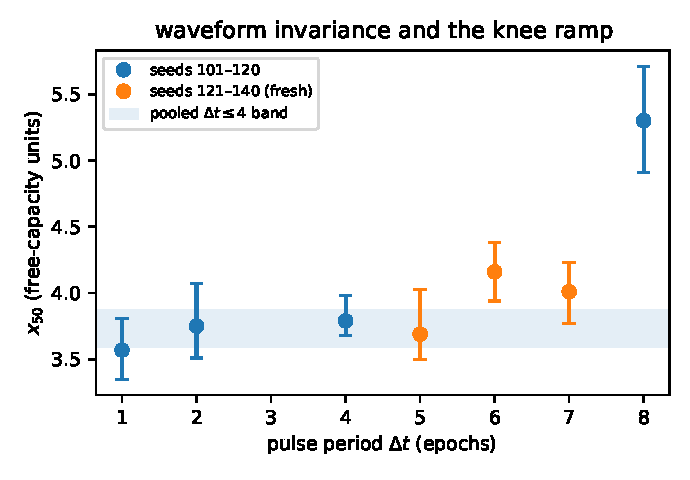
\includegraphics[width=0.62\textwidth]{fig5_knee_ramp.pdf}
\caption{Waveform invariance and the knee ramp: $x_{50}$ vs.\ pulse period,
two seed cohorts, with the pooled $\dt\le4$ band. Invariance holds through
$\dt=5$; the wall lifts along a graded ramp to $\dt=8$.}\label{fig:knee}
\end{figure}
\begin{figure}[h]\centering
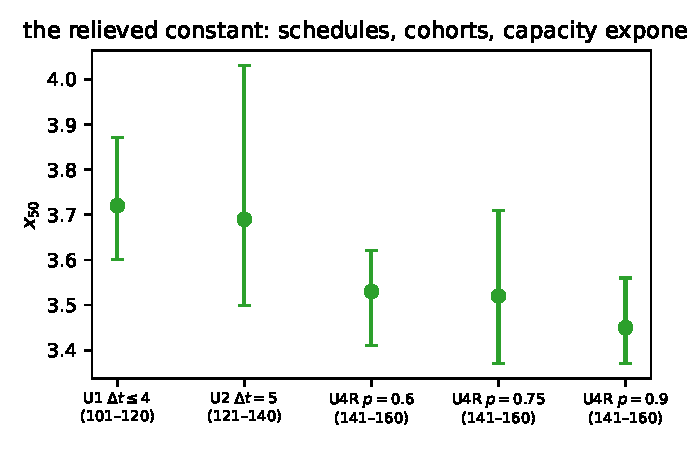
\includegraphics[width=0.62\textwidth]{fig6_relieved_constant.pdf}
\caption{The relieved constant across schedules, independent seed cohorts,
and exterior capacity exponents $p\in\{0.6,0.75,0.9\}$.}\label{fig:relieved}
\end{figure}
\begin{figure}[h]\centering
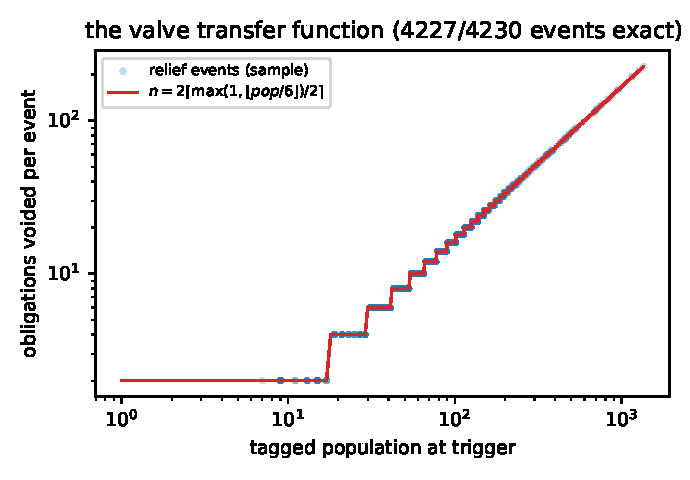
\includegraphics[width=0.62\textwidth]{fig7_transfer_function.pdf}
\caption{The valve transfer function, event level: obligations voided per
relief event vs.\ tagged population at trigger, with the exact law of
Eq.~\ref{eq:law} (4227/4230 events exact; the three exceptions are
exhaustion-side).}\label{fig:transfer}
\end{figure}
\begin{figure}[h]\centering
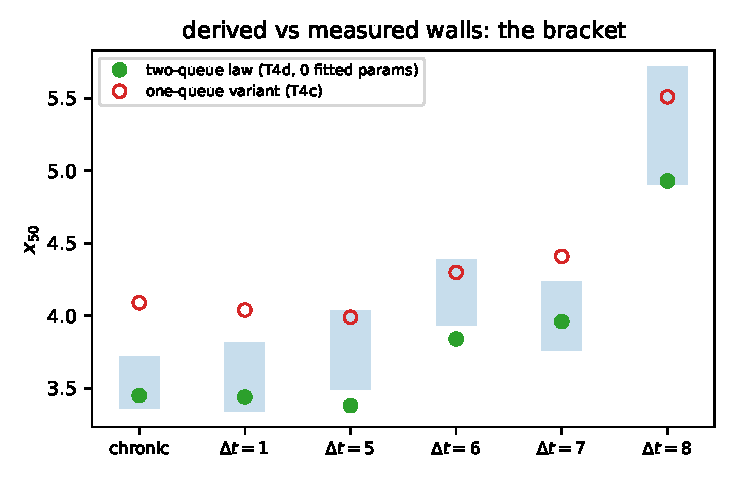
\includegraphics[width=0.68\textwidth]{fig8_bracket.pdf}
\caption{Derived vs.\ measured walls. Bars: engine 95\% CIs. Filled points:
the two-queue law (zero fitted parameters). Open points: the one-queue
variant. Every measured wall lies inside the two-variant bracket.}
\label{fig:bracket}
\end{figure}

\end{document}
